\section{Vientos Estelares}
\section{Choques}
\section{Frentes de Ionización}
\section{Regiones HII}
Las regiones HII se forman cuando una estrella masiva, de tipo espectral
O ó B temprana, ioniza el gas que se encuentra a su alrededor. El gas
ionizado se encuentra en equilibrio térmico, a una temperatura del
orden de $10^4~K$. El principal proceso de calentamiento es la
radiación de la estrella central, mientras que el enfriamiento se da
principalmente por la recombinación de líneas prohibidas y por emisión
libre-libre.

\section{Modelo Genérico de los Choques de Proa}
\label{sec:Modelo-generico}
Para este trabajo consideramos en general dos modelos de
interacción  de vientos:
\begin{itemize}
\item Una fuente localizada en el origen que emite un viento esférico
  que puede ser isotrópico o anisotrópico (figura
  \ref{fig:isotropic-aniso}) no acelerado que interactúa con el viento
  esférico isotrópico de otra fuente que se encuentra a una distancia
  $D$ de la primera(figura \ref{fig:crw-esquema})
\item Una fuente localizada en el origen que emite un viento esférico
  isotrópico no acelerado que interactúa con un viento plano paralelo
  no acelerado y densidad constante (figura )
\end{itemize}
El sitema en su conjunto tiene simtería cilíndrica.
\begin{figure}
  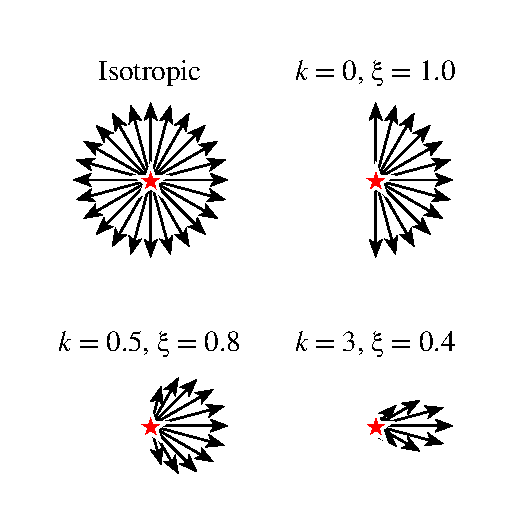
\includegraphics[width=0.5\linewidth]{./Figures/anisotropic-arrows}
  \label{fig:isotropic-aniso}
  \caption{Representación esquemática de vientos con diferentes
    anisotropías:
    Arriba izquierda: Viento isotrópico esférico. Arriba derecha: viento
    isotrópico hemisférico. Abajo: Vientos anisotrópicos donde el
    parámetro $k$ indica el grado de anisotropía (ver sección
    \ref{sec:hipersonica})}
\end{figure}
\begin{figure}
  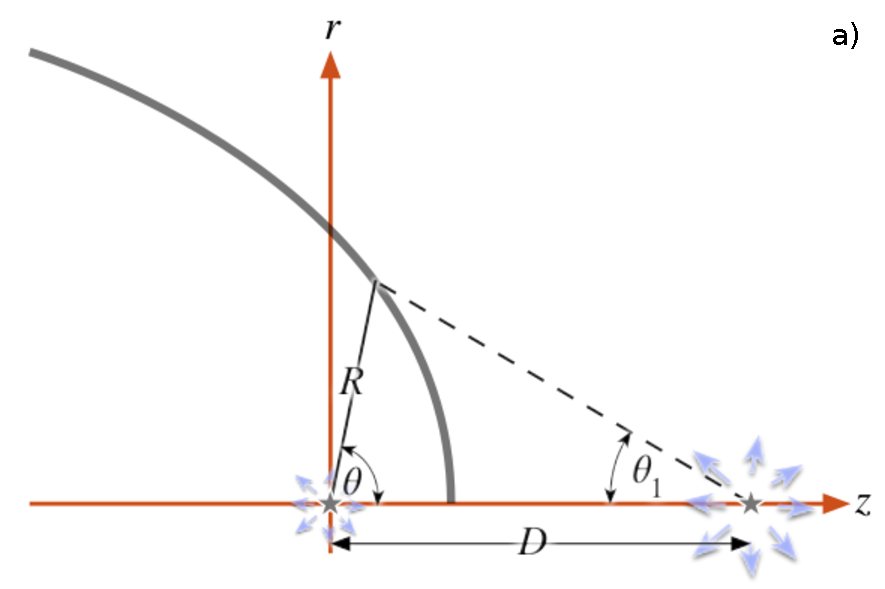
\includegraphics[width=0.5\linewidth]{./Figures/bowshock-crw-variables}
  \label{fig:crw-esquema}
\end{figure}

\subsection{Radios ``Característicos''}
\label{sec:char-rad}
Las cantidades medibles que nos ayudan a caracterizar un choque de proa las
llamamos ``Radios característicos'' (ilustrados en la figura
\ref{fig:char-radii}):
\begin{itemize}
\item Radio del choque en la dirección del eje de simetría del sistema.
  Denotado como $R_0$
\item Radio en dirección perpendicular al eje de simetría del sistema.
  Denotado como $R_{90}$
\item Radio de curvatura en la ``nariz'' del choque de proa. Denotado
  como$ R_c$
\end{itemize}

\begin{figure}
  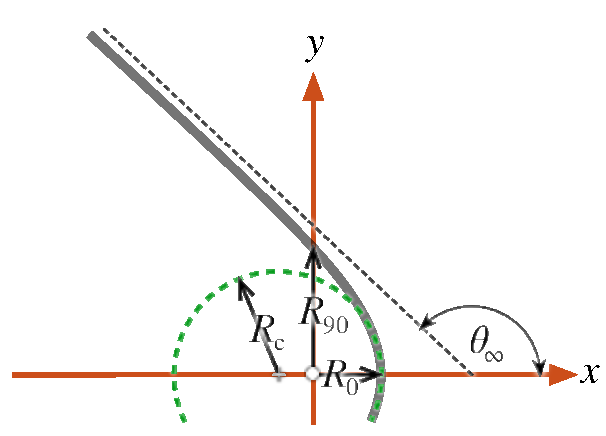
\includegraphics[width=\linewidth]{./Figures/characteristic-radii}
  \label{fig:char-radii}
  \caption{Representación esquemática de los radios característicos
  de un choque de proa}
\end{figure}.
Para este trabajo resulta útil hacer una noramlización de los radios
característicos u otros radios, para que las mediciones que obtengamos
sean adimensionales. De esta forma, podemos hacer la normalización con
la distancia $D$, o bien con $R_0$, dependiendo de qué tipo de
normalización resulte más conveniente. En el primer caso expresamos
explícitamente el cociente (e.g $\frac{R_0}{D}$, $\frac{R_c}{D}$,
$\frac{R_{90}}{D}$), y en el segundo caso añadiremos una tilde al
radio en cuestión (e.g $\tilde{R}_c$, $\tilde{R}_{90}$).

\section{Aproximación Hipersónica}
\label{sec:hipersonica}


\section{Proyección en el Plano del Cielo}
\label{sec:projection}

Para un choque de proa que es la vez geom\'etricamente delgado y
\'opticamente delgado, \'unicamente se observa el borde de \'este por
abrillantamiento al limbo, por lo tanto, sua orientaci\'on respecto a
la l\'inea de visi\'on modifica su forma respecto a la forma real del
choque. Para ello, rotamos el sistema de referencia del choque de proa
en coordenadas cartesianas, denotado por $(x, y, z)$, por un \'angulo
que llamamos \textit{inclinaci\'on}, denotado por $i$, en el plano $xz$,
de modo que la transformaci\'on entre el sistema de refencia del choque
y el sistema de referencia del plano del cielo, denotado por
$(x', y', z')$ queda como sigue:

\begin{align}
  \left(
  \begin{array}{c}
    x' \\ y' \\ z'
  \end{array}
  \right) &=
  \left(
  \begin{array}{c}
    x\cos i - z\sin i \\ y' \\ z\cos i + x\sin i
  \end{array}
  \right)
  \label{eq:rotation}
\end{align}

Por otro lado, la forma tridimensional del choque de proa viene dado por:

\begin{align}
  \left(
  \begin{array}{c}
    x \\ y \\ z
  \end{array}
  \right) &=
            R(\theta)\left(
            \begin{array}{c}
              \cos\theta \\
              \sin\theta\cos\phi \\
              \sin\theta\sin\phi
            \end{array}
            \right)
\end{align}
La relaci\'on entre ambos sistemas de referencia se ilustra en la figura
\ref{fig:reference}.

\begin{figure}
  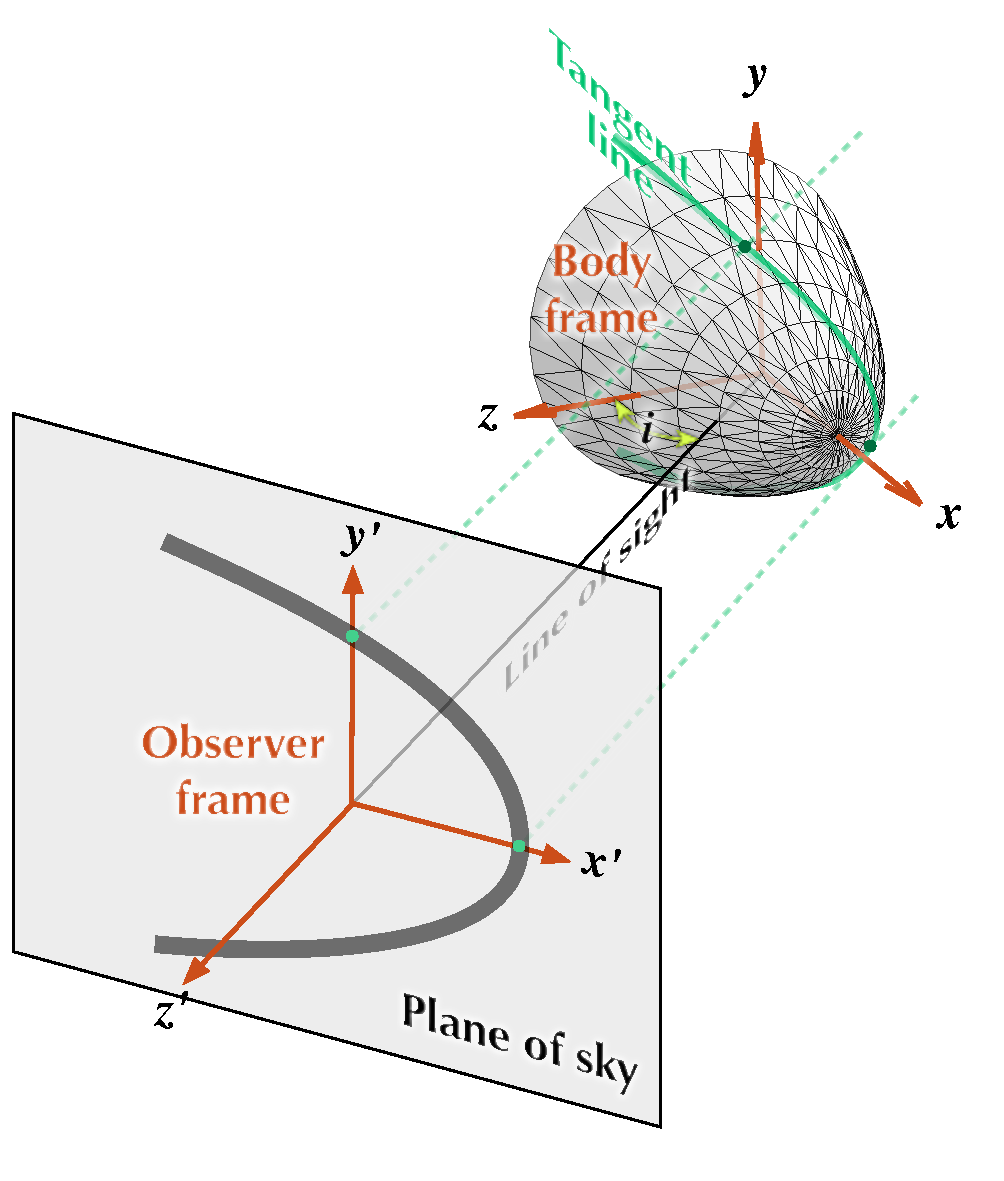
\includegraphics[width=\linewidth]{./Figures/projection-pos}
  \label{fig:reference}
  \caption{Sistema de referencia del choque vs sistema de referencia del
    plano del cielo. Los ejes $x'$ y $y'$ se encuentran en el plano del
    cielo, mientras el eje $z'$ es paralelo a la línea de visión.
    Solo la regi\'on del choque cuya tangente sea paralela a la l\'inea
    de visión será visible por abrillantamiento al limbo.}
\end{figure}

\subsection{Vectores normal y tangente a la superficie}

Si definimos los vectores $\hat{n}$ y $\hat{t}$, como los vectores
normal y tangente a la superficie, respectivamente para $\phi$ constante.
En el caso $\phi = 0$ (figura \ref{fig:unit-vec}), ambos vectores se encuentran
en el plano $xy$ y es fácil mostrar que:

\begin{align}
  \hat{t}_0 =
  \left(
  \begin{array}{c}
    -\cos\alpha \\
    \sin\alpha \\
    0
  \end{array}
  \right)
  \quad \mathrm{y} \quad
  \hat{n}_0 =
  \left(
  \begin{array}{c}
    \sin\alpha \\
    \cos\alpha \\
    0
  \end{array}
  \right)
  \label{eq:unit-vec}
\end{align}

Donde:
\begin{align}
  \tan\alpha = -\frac{dy}{dx} = \frac{1+\omega\tan\theta}{\tan\theta-\omega}
\end{align}
y:
\begin{align}
  \omega(\theta) = -\frac{1}{R}\frac{dR}{d\theta} 
\end{align}

Para otros valores de $\phi$, basta con hacer una rotación de las ecuaciones
(\ref{eq:unit-vec}) alrededor del eje $x$. Para la conversión al sistema de
referencia del plano del cielo se utiliza la ecuación (\ref{eq:rotation}):

\begin{align}
  \hat{n}' &= \frac{1}{\left(1 + \omega^2\right)^{1/2}} \\
           & \times \left(
             \begin{array}{c}
               (\cos\theta+\omega\sin\theta)\cos i-(\sin\theta-\omega\cos\theta)\sin i\sin\phi\\
               (\sin\theta-\omega\cos\theta)\cos\phi \\
               (\cos\theta+\omega\sin\theta)\sin i+(\sin\theta-\omega\cos\theta)\sin\phi\cos i
             \end{array}
                    \right) \\
    \hat{t}' &= \frac{1}{\left(1 + \omega^2\right)^{1/2}} \\
           & \times \left(
             \begin{array}{c}
               -(\sin\theta-\omega\cos\theta)\cos i-(\cos\theta+\omega\sin\theta)\sin i\sin\phi\\
               (\cos\theta+\omega\sin\theta)\cos\phi \\
               -(\cos\theta+\omega\sin\theta)\sin i+(\sin\theta-\omega\cos\theta)\sin\phi\cos i
             \end{array}
             \right) 
\end{align}


\begin{figure}
  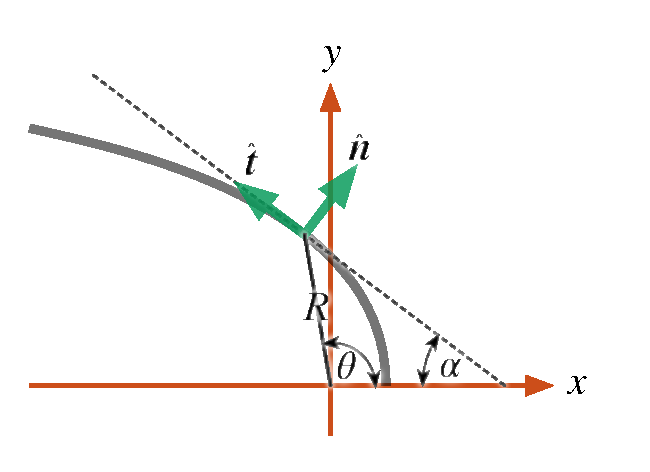
\includegraphics[width=0.8\linewidth]{./Figures/bowshock-unit-vectors}
  \label{fig:unit-vec}
  \caption{Vectores unitarios normal y tangente a la superficie $R(\theta)$
    en un plano de azimuth $\phi$ constante.}
\end{figure}


\subsection{Línea tangente}

Debido a que el choque es \'opticamente delgado y geom\'etricamente
delgado, solo la regi\'on del choque cuya tangente sea paralela a la
l\'inea de visi\'on ser\'a visible. Esto corresponde a una curva que
denominamos \textit{l\'inea tangente}, que debe cumplir con la siguiente
condición:

\begin{align}
  \hat{n}'\boldsymbol{\cdot} \hat{z}' = 0
\end{align}

Denotamos como $\phi_T$ al ángulo azimutal que cumple la condición anterior
para una inclinación dada, en función del ángulo polar $\theta$:
\begin{align}
  \sin\phi_T = \tan i\tan\alpha = \tan i\frac{1+\omega\tan\theta}{\omega-\tan\theta}
  \label{eq:phi-tan}
\end{align}
De esta manera, la forma de la línea tangente del choque de proa, a la que llamamos
\textit{forma proyectada} viene dada por:

\begin{align}
  \left(
  \begin{array}{c}
    x'_T \\
    y'_T \\
    z'_T
  \end{array}
  \right) =
  R(\theta)\left(
  \begin{array}{c}
    \cos\theta\cos i - \sin\theta\sin\phi_t\sin i \\
    \sin\theta\left(1-\sin^2\phi_T\right)^{1/2} \\
    \cos\theta\sin i + \sin\theta\sin\phi_T\cos i
  \end{array}
  \right) \label{eq:proj-shape}
\end{align}
En el caso general, $z'_T$ no es una función lineal de $x'_t$ y $y'_T$, por lo que
la línea tangente no se encuentra en un plano.

La forma aparente $(x'_t, y'_T)$  de la línea tangente también puede escribirse
en coordenadas polares $(R', \theta')$, donde:
\begin{align}
  R'(\theta) = \left(x'_t^2 + y'_T^2\right)^{1/2} & \mathrm{y} & \tan\theta' = \frac{y'_T}{x'_T}
  \label{eq:polar}
\end{align}
Es de notar a su vez que la ecuación (\ref{eq:phi-tan}) no tiene solución para valores
arbitrarios de $\theta$ y de la inclinación, puesto que se requiere que
$\left|\sin\phi_T\right| < 1$. Por tanto, la línea tangente solo existe para valores
de $\theta$ tales que $\theta < \theta_0$ donde $\theta_0$ es el valor de $\theta$ en
el eje de simetría de la línea tangente proyectada $(\theta'(\theta_0)) = 0$ y que se
obtiene de la siguiente ecuación implícita:
\begin{align}
  \tan\theta_0 = \frac{|\tan i| + \omega(\theta_0)}{1 - \omega(\theta_0)|\tan i|}
  \label{eq:th-0}
\end{align}
Esto implica que si el choque de proa es suficientemente ``abierto''
$(\alpha > \alpha_{min})$, entonces para inclinaciones tales que
$|i| > 90^\circ - \alpha_{min}$ no existirá la línea tangente para ningún valor de $\theta$,
es decir, el choque de proa se encontrará sufientemente ``de cara'' como para que ya no
parezca un chouque de proa para el observador.

\subsection{Radios característicos en el plano del cielo}

En orden de comparar la forma $R(\theta)$ con observaciones, es útil definir los radios
característicos $R'_0$ y $R'_{90}$, donde $R'_0$ es el radio del eje de simetría aparente
y $R'_{90}$ es el radio aparente en la dirección perpendicular a $R'_0$. Es decir
$R'_0 = x'_T(y'_t=0)$ y $R'_{90} = y'_t(x'_t = 0)$. Utilizando las ecuaciones
(\ref{eq:phi-tan}) y (\ref{eq:proj-shape}) encontramos que:
\begin{align}
R'_0 = R(\theta_0)\cos(\theta_0 + i)
\label{eq:R0p}
\end{align}
Donde $\theta_0$ es la solución de la ecuación (\ref{eq:th-0}), y
\begin{align}
  R'_{90} = R(\theta_{90})\sin\theta_{90}\left(1-\sin^2\phi_T(\theta_{90})\right)^{1/2}
  \label{eq:R90p}
\end{align}
donde $\theta_{90}$ es la solución de la siguiente ecuación implícita:
\begin{align}
  \cot\theta_{90} = \frac{1 - \left(1+\omega(\theta_{90})^2\sin^22i\right)^{1/2}}
  {2\omega(\theta_{90})\cos^2i}
  \label{eq:th90}
\end{align}

\section{Cuádricas de Revolución}

\newcommand\Sin{\ensuremath{\mathcal{S}}}
\newcommand\Cos{\ensuremath{\mathcal{C}}}
\newcommand\Cot{\ensuremath{\mathcal{T}}}


En el caso general es difícil encontrar la forma aparente para un choque de
proa siguiendo el formalismo desarrollado en la sección anterior, por lo que
optamos por aproximar la forma éstos con una de las superficies más simples:
las \textit{cuádricas de revolución}, que son superficies de revolución de
las curvas cónicas. Dado el modelo general descrito en la sección
\ref{sec:Modelo-generico}, haremos algunas restricciones para las superficies
cuádricas que utilizaremos en este trabajo:
\begin{itemize}
  \item El eje focal se encuentra alineado con el eje $x$
  \item La posición del foco de la superficie cuádrica no necesariamente coincide
    con la posición de la fuente
  \item En el caso de las hipérbolas, solo tomamos una de las ramas de ésta.
\end{itemize}
Implementando dichas restricciones, utilizamos la representación paramétrica de
las curvas cónicas en términos de un parámetro adimensional denotado con la letra
$t$ de manera general:
\begin{align}
  x &= a\Cos(t) + x_0\\
  y &= b\Sin(t) 
\end{align}
Donde:
\begin{align}
  \Cos(t) =\left\lbrace
  \begin{array}{lr}
    \cos{t} & \theta_c > 0\\
    -\cosh{t} & \theta_c < 0        
  \end{array}\right. \\
  \Sin(t) = \left\lbrace
  \begin{array}{lr}
    \sin{t} & \theta_c > 0\\
    \sinh{t}  & \theta_c < 0
  \end{array} \right. \\
  x_0 &= R_0 \mp a \label{eq:x0} 
\end{align}
Donde $a$ y $b$ representan la longitud del semi-eje mayor y menor, respectivamente (Figura \ref{fig:conics}).
$x_0$ representa la distancia entre el centro de la cónica y el origen. 
$\theta_c$ es un parámetro que está relacionado con la excentricidad y que en este
trabajo sustituye a ésta y que están relacionadas por la siguiente expresión:
\begin{align}
  \tan\theta_c = \pm\sqrt{\left|1-e^2\right|}
\end{align}
Tomamos el signo positivo cuando la cantidad dentro de las barras de valor absoluto es
positiva y viceversa (Figura \ref{fig:conics-family}). También podemos definirlo en
términos de los parámetros de las cónicas:

\begin{align}
  \tan\theta_c = \pm \frac{b}{a} \label{eq:thc}
\end{align}
Siguiendo la convención de que el signo positivo corresponde a elipses, negativo a
hipérbolas y cero para las parábolas.

\begin{figure}
  \begin{tabular}{cc}
    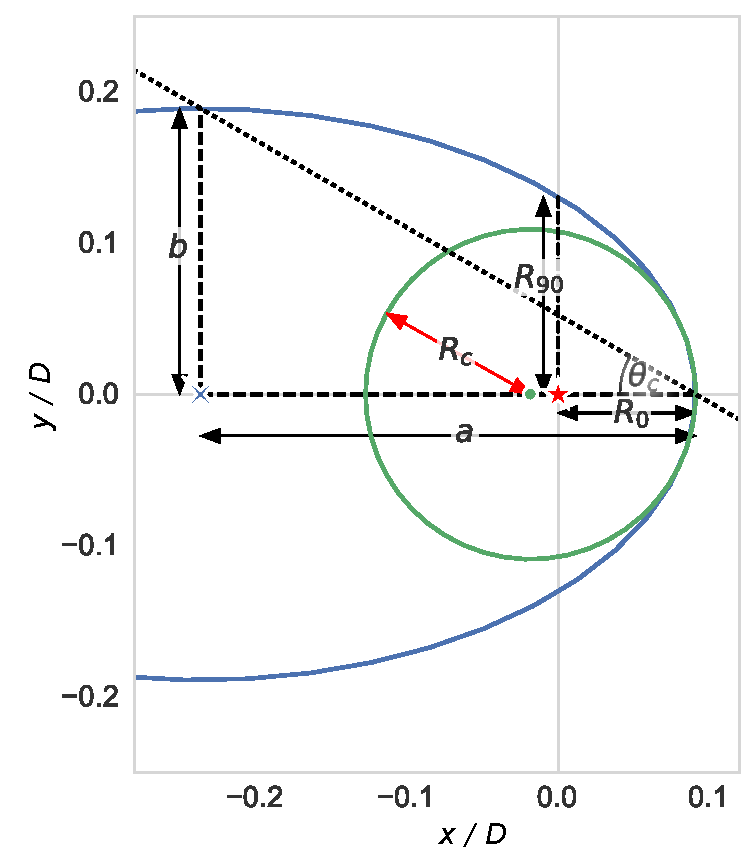
\includegraphics[width=0.5\linewidth]{./Figures/ellipse_edited} &
    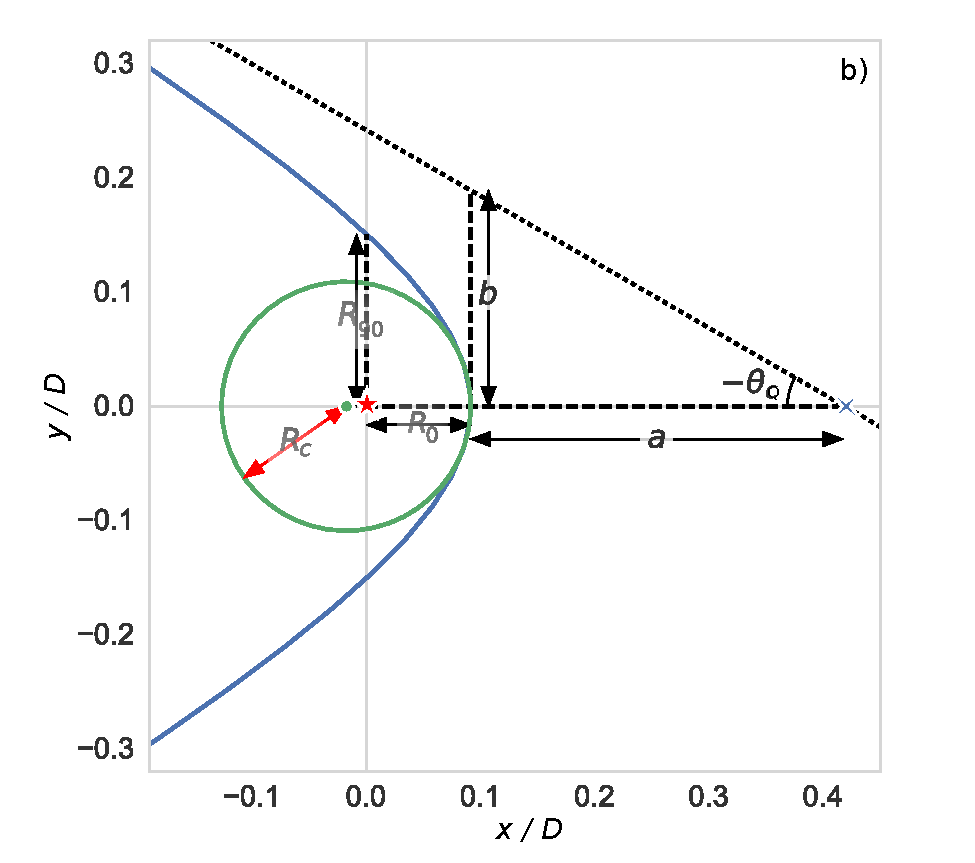
\includegraphics[width=0.5\linewidth]{./Figures/hyperbola_edited}
  \end{tabular}
  \label{fig:conics}
  \caption{Representación esquemática de: Izquierda: Elipse. Y, derecha: Hipérbola.
  En ambos casos se ilustran los parámetros relevantes de éstas y los radios característicos}
\end{figure}

\begin{figure}
  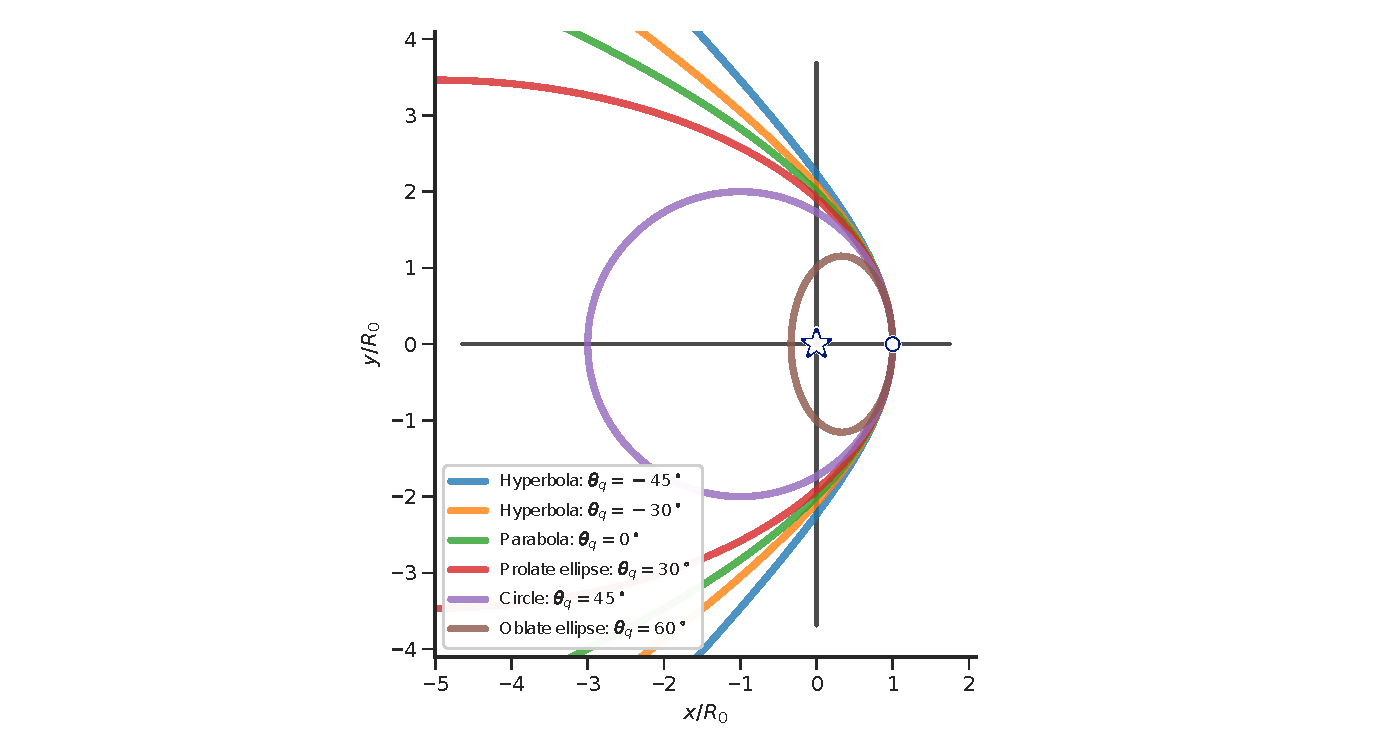
\includegraphics[width = \linewidth]{./Figures/conic1}
  \label{fig:conics-family}
  \caption{Familia de curvas cónicas, donde el valor del parámetro $\theta_c$ varía desde
    $\theta_c <0$ (hipérbolas) hasta $\theta_c > 0$ (elipses). Casos especiales son $\theta_c = 0$
  (parábola) y $\theta_c = 45^\circ$ (círculo). Este parámetro sustituye en este trabajo a la excentricidad.}
\end{figure}

\subsection{Radios Característicos}

Para que las curvas cónicas den una buena aproximación a la forma de un choque de proa dado, necesitamos saber
calcular los radios característicos para éstas. A partir de la descripción de estos en la sección
\ref{sec:char-rad} podemos encontrar expresiones para cada uno de éstos en términos de los parámetros de las
cónicas:

\begin{align}
  R_c &= \frac{b^2}{a} \label{eq:R-curv-conic}\\
  R_{90} &= b\left[\pm\left(1 - \frac{(R_0 - a)^2}{a^2}\right)\right]^{1/2} \label{eq:R90-conic}
\end{align}
$R_0$ es independiente de los parámetros de las cónicas, por tanto, en
esta sección nos será útil normalizar con este radio. De esta forma,
podemos invertir las siguientes ecuaciones:

\begin{align}
  \tilde{a} &= \pm\frac{\tilde{R}_c}{2\tilde{R}_c - \tilde{R}_{90}^2} \\
  \tilde{b} &= \frac{\tilde{R}_c}{\left|2\tilde{R}_c - \tilde{R}_{90}^2\right|^{1/2}}\\
  \tan\theta_c &= \pm\left|2\tilde{R}_c - \tilde{R}_{90}^2\right|^{1/2}
\end{align}
Nótese que la cantidad $T_c\equiv 2\tilde{R}_c - \tilde{R}_{90}^2$ nos sirve como discriminante para
distinguir el tipo de curva cónica que mejor ajusta a un choque de proa dado.

\subsection{Proyección en el plano del cielo}

El objetivo de esta sección es obtener la forma proyectada de las cuádricas de revolución,
puesto que son una aproximación buena y mucho más sencilla a la forma real de un choque de
proa.
La forma tridimensional de las cuádricas de revolución viene dada por:

\begin{align}
  x &= a\Cos(t) - x_0 \\
  y &= b\Sin(t)\cos\phi \\
  z &= b\Sin(t)\sin\phi
\end{align}

Siguiendo el procedimiento mostrado en la sección \ref{sec:projection} calculamos el ángulo
azimutal $\phi$ que cumple con el criterio de ser tangente al la línea de visión:

\begin{align}
  \sin\phi_T = \frac{b}{a}\tan i\Cot(t) 
\end{align}
Donde:
\begin{align}
  \Cot(t) = \left\lbrace
  \begin{array}{lr}
    \cot t & if~\theta_c > 0 \\
    \coth t & if~\theta_c < 0 
  \end{array}
  \right.
\end{align}

Podemos movernos a otro sistema de referencia $(X, Y)$ centrado en el origen, donde
$X = x - x_0$ y $Y =y$. En este sistema, utilizamos la ecuación (\ref{eq:rotation})
para obtener la forma aperente de una cuádrica dada:

\begin{align}
  X'_T &= \frac{\Cos(t)}{a\cos i}\left(a^2\cos^2 i \pm b^2\sin^2 i\right)
  \label{eq:x-prime-proj}\\
  Y'_T &= b\Sin(t)\left(1 - \frac{b^2}{a^2}\tan^2 i\Cot^2(t)\right)^{1/2}
  \label{eq:y-prime-proj}
\end{align}

Se espera que la forma proyectada de una cuádrica dada sea otra cuárica del mismo
tipo, por lo que es posible escribir las ecuaciones (\ref{eq:x-prime-proj}) y
(\ref{eq:y-prime-proj}) de la siguiente manera: 

\begin{align}
  X'_T &= a'\Cos(t') \\
  Y'_T &= b'\Sin(t')
\end{align}
Donde:
\begin{align}
  a' &= \left(a^2\cos^2 i \pm \b^2\sin^2 i\right)^{1/2} \label{eq:a-prime}\\
  b' &= b \label{eq:b-prime}\\
  \Cos(t') &= \frac{a'\Cos(t)}{a\cos i} \\
  \Sin(t') &= \left(1 - \Cos^2(t')\right)^{1/2}
\end{align}

También implica que para encontrar los radios característicos en el sistema de
referencia del observador solamente tenemos que sustituir $a$ y $b$ por $a'$ y
$b'$ en las ecuaciones (\ref{eq:x0}), (\ref{eq:R-curv-conic}), (\ref{eq:R90-conic})
y (\ref{eq:thc}):

\begin{align}
  R'_0 &= \pm a' +x_0\cos i\\
  R'_c &= \frac{b'^2}{a'}\\
  \tan\theta'_c &= \frac{b'}{a'} \\
  R'_{90} &= \left(2R'_c \mp \tan^2\theta'_c\right)^{1/2}
\end{align}

Utilizando las ecuaciones (\ref{eq:x0}), (\ref{eq:a-prime}) y (\ref{eq:b-prime}),
utlizando la definición $D' = D\cos i$ e introduciendo la función
$f(i;\theta_c)\equiv \left(1 \pm \tan^2\theta_c\tan^2i\right)^{1/2}$ obtenemos
ecuaciones explícitas para los radios característicos en el sistema de referencia
del plano del cielo en términos de la inclinación:

\begin{align}
  \frac{q'}{q} &= 1 \pm \tilde{R}_c\cot^2\theta_c\left(f(i;\theta_c) - 1\right) \\
  \tilde{R}'_c &= \frac{\tilde{R_c}}{\cos^2if(i;\theta_c)\frac{q'}{q}} \\
  \tan\theta'_c &= \frac{\tan\theta_c}{\cos if(i;\theta_c)} \\
  \tilde{R}'_{90} &= \left(\frac{2\tilde{R}_cf(i;\theta_c) \mp
                  \tan^2\theta_c\frac{q'}{q}}{q'/q}\right)^{1/2}\frac{\sec i}{f(i;\theta_c)}
\end{align}

Cuando $\tilde{R}'_{90}$ es medible, entonces es posible hacer diagramas de diagnóstico como
el de la figura \ref{fig:diagnostic} para comparar con observaciones, independientemente de
cualquier modelo de choques de proa.

\begin{figure}
  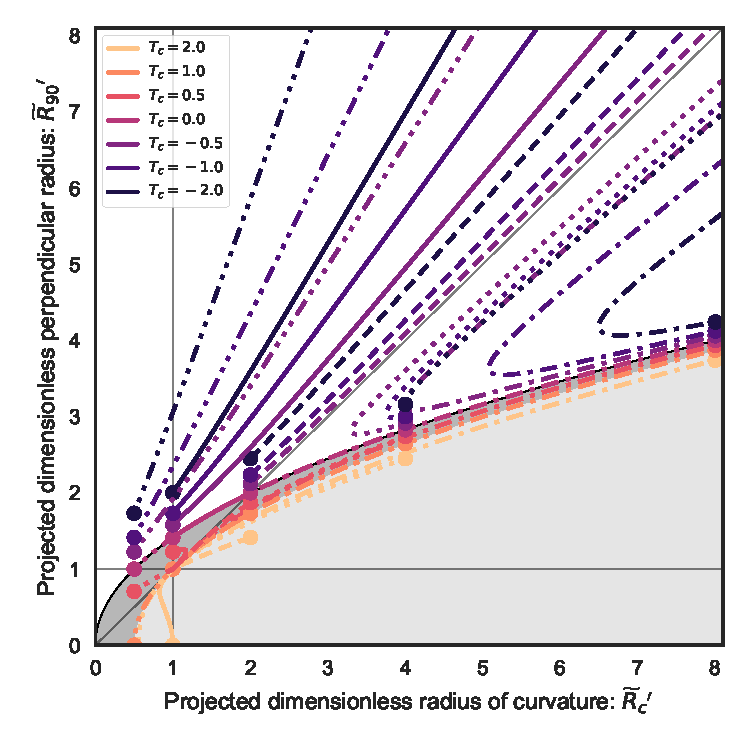
\includegraphics[width=0.5\linewidth]{./Figures/projected-R90-vs-Rc}
  \label{fig:diagnostic}
  \caption{Diagrama de diagnóstico $\tilde{R}'_{90}$ vs $\tilde{R}'_c$ para las cuádricas
    de revolución. En la región sin sombrear se representan las superficies abiertas
    (hiperboloides, $\theta_c <0$), mientras que la región más oscura representa  a
    elipsoides prolatos  $(0 < \theta_c < 45^\circ)$ y la región poco sombreada a
    elipsoides oblatos $(\theta_c > 45^\circ)$}
\end{figure}

Buscamos adjuntar el paper ``quadrics bowshock''
